\section*{The DFT on Real-World Sounds}

\subsection*{The DFT on Audio}

So far we have used contrived examples to get a better understanding of how the DFT works on both periodic and
aperiodic samples.  Let us put it all together and examine an unknown piece of audio.  We will look at the magnitude
and phase response of the samples and draw some conclusions about the original audio file.  Later in this section, I
will reveal the origin of the audio file and we can reexamine our conclusions.  Figure \ref{fig:unknown} shows the 
time domain representation, magnitude response and phase response of this signal.

\begin{figure}[h]
	\caption{The time domain, magnitude response and phase response plots of an unknown audio signal}
	\label{fig:unknown}
	\begin{center}
		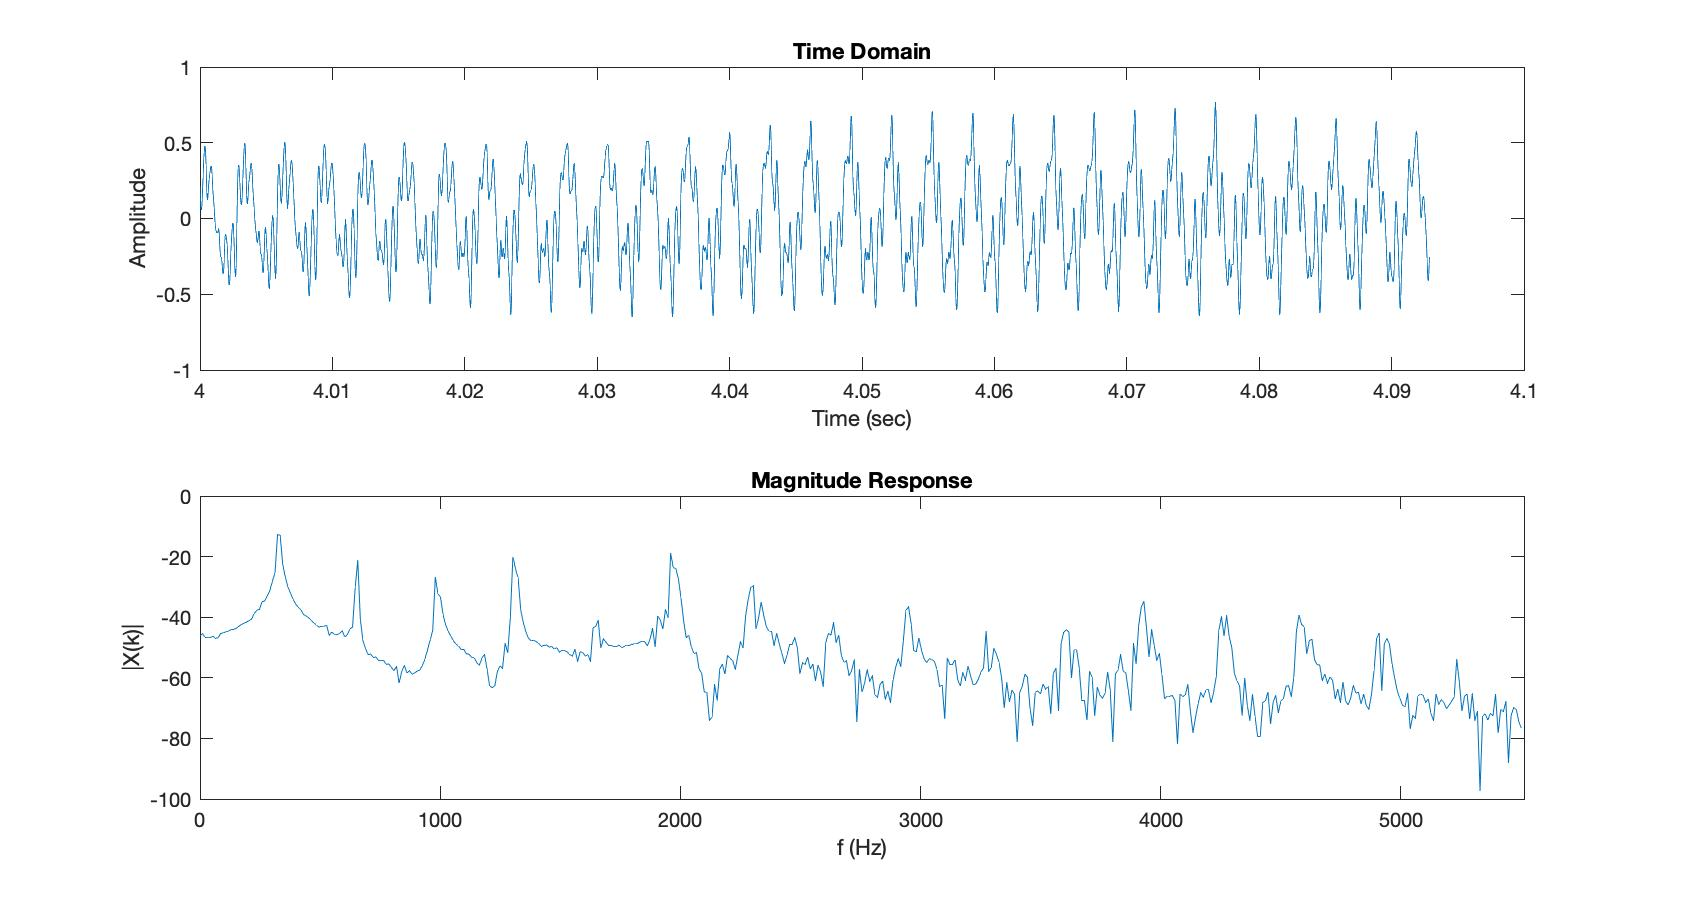
\includegraphics[scale = 0.28]{violin.jpg}
	\end{center}
\end{figure}

If we look at the time domain representation of the sound, we can see a repeating peak of the same shape.  This
strongly suggests strong harmonic content because repetitions in the time domain produce a fundamental whose
frequency is the number of repetitions per second.  The period of the shape is roughly 0.003 seconds or a third of
a hundredth of a second.  With a period of 0.003 seconds, we would assume that we would have a fundamental
roughly around 330Hz.  Though its a little difficult to tell, the magnitude response also has a peak near 330Hz
which confirms are intuition about the presence of 330Hz in the sound.  Observe as well how the time domain
waveform maintains the same period but has slight differences in each repetition and particularly over time.  We
can see the amplitude of the time domain waveform grows over the span of that tenth of a second.  These
slight variations suggest a real instrument as opposed to an electronic waveform like a sawtooth wave which
would have identical repetitions.  Those slight differences as the sound progresses through time give a real
instrument that ``naturalness" that distinguishes it from electronic instruments.

We will ignore the phase response for this analysis; however, the magnitude response contains important
information.  Notice the succession of peaks equidistant apart.  We can see them at roughly 330Hz, 660Hz,
990Hz, etc.  All these subsequent peaks after 330Hz represent partials of the fundamental 330Hz which
roughly corresponds to an ``E4".  Though the whole magnitude spectrum is not shown, we can see a
relatively rich harmonic spectrum where many of the harmonics are present.  Interestingly though, the
fifth harmonic at 1650Hz is not as prominent.  Based on this magnitude spectrum, it is likely that this
is a real instrument that produces lots of harmonics.  

It turns out that this is a violin playing an ``E4".  Both the time domain and the magnitude spectrum suggested
an instrument playing a note at ``E4".  Violins are instruments with rich spectrum.  The variation in the peak
height help give the violin its unique sound.  If we were to take the DFT of the next series of samples, we would
see slight changes in the peak height.  The slight evolution of harmonics as well as several inharmonic partials
give the violin the wonderful sound we have come to love.

\subsection*{Time Resolution vs. Frequency Resolution}

The DFT provides a straightforward way to convert audio from the time domain to the frequency domain.  Many
programming languages and audio applications have optomized algorithms that handle all of the computation.
The user typically decides what samples will be processed and how many.  The number of samples $N$ is an important
consideration.  Recall that the number of frequency bins is equivalent to the number of samples taken and that the
distance between each bin is $f_s/N$.  The larger $N$ is, the more frequency bins and the more finely parsed the frequency spectrum is.  $N$ plays an important role in separating frequencies, particularly lower frequencies.  Our perception of intervals is based on the ratio betweendistinct frequencies.  For example, a ratio of 2:1 expresses an
octave and holds true whether the frequencies are 40Hz and 20Hz or 20000Hz and 10000Hz.  Lower notes are 
clustered closer together in frequency while higher notes are spaced farther.  By contrast, the 
frequency bins of the DFT are linear.  The same distance separates each bin.  Consider a standard sampling 
rate of $f_s = 44100$Hz and a $N = 1024$.  The distance between each bin is approximately 43Hz, leading to 
bins of 0Hz, 43Hz, 86Hz, etc.  The frequency 43Hz corresponds roughly to the note F1 and 86Hz corresponds
roughly to F2.  That is a full octave separating those two frequency bins!  

To increase the frequency resolution, we can increase the number of samples we process.  This is an easy solution,
but it comes at a cost.  The more samples $N$ we take, the poorer our time resolution becomes.  We generally use
the DFT on short slices of audio so we can get a snapshot of the frequency content.  The larger $N$ becomes, the
wider that snapshot is.  For audio with a slow changing spectra, this is not a problem.  For audio with fast moving
spectra, the $N$ samples can contain many musical moments, making it harder to interpret the magnitude response.

As an example, consider a larger $N$ for the violin E4 excerpt we saw earlier.  Let's set $N$ to 30000, significantly larger
than the $N = 4096$ samples we took to plot Figure \ref{fig:unknown}.  This moment comes from a later portion in
the audio file and is plotted in Figure \ref{fig:violinTwoNotes}.

\begin{figure}[h]
	\caption{The time domain, magnitude response and phase response plots of a violin}
	\label{fig:violinTwoNotes}
	\begin{center}
		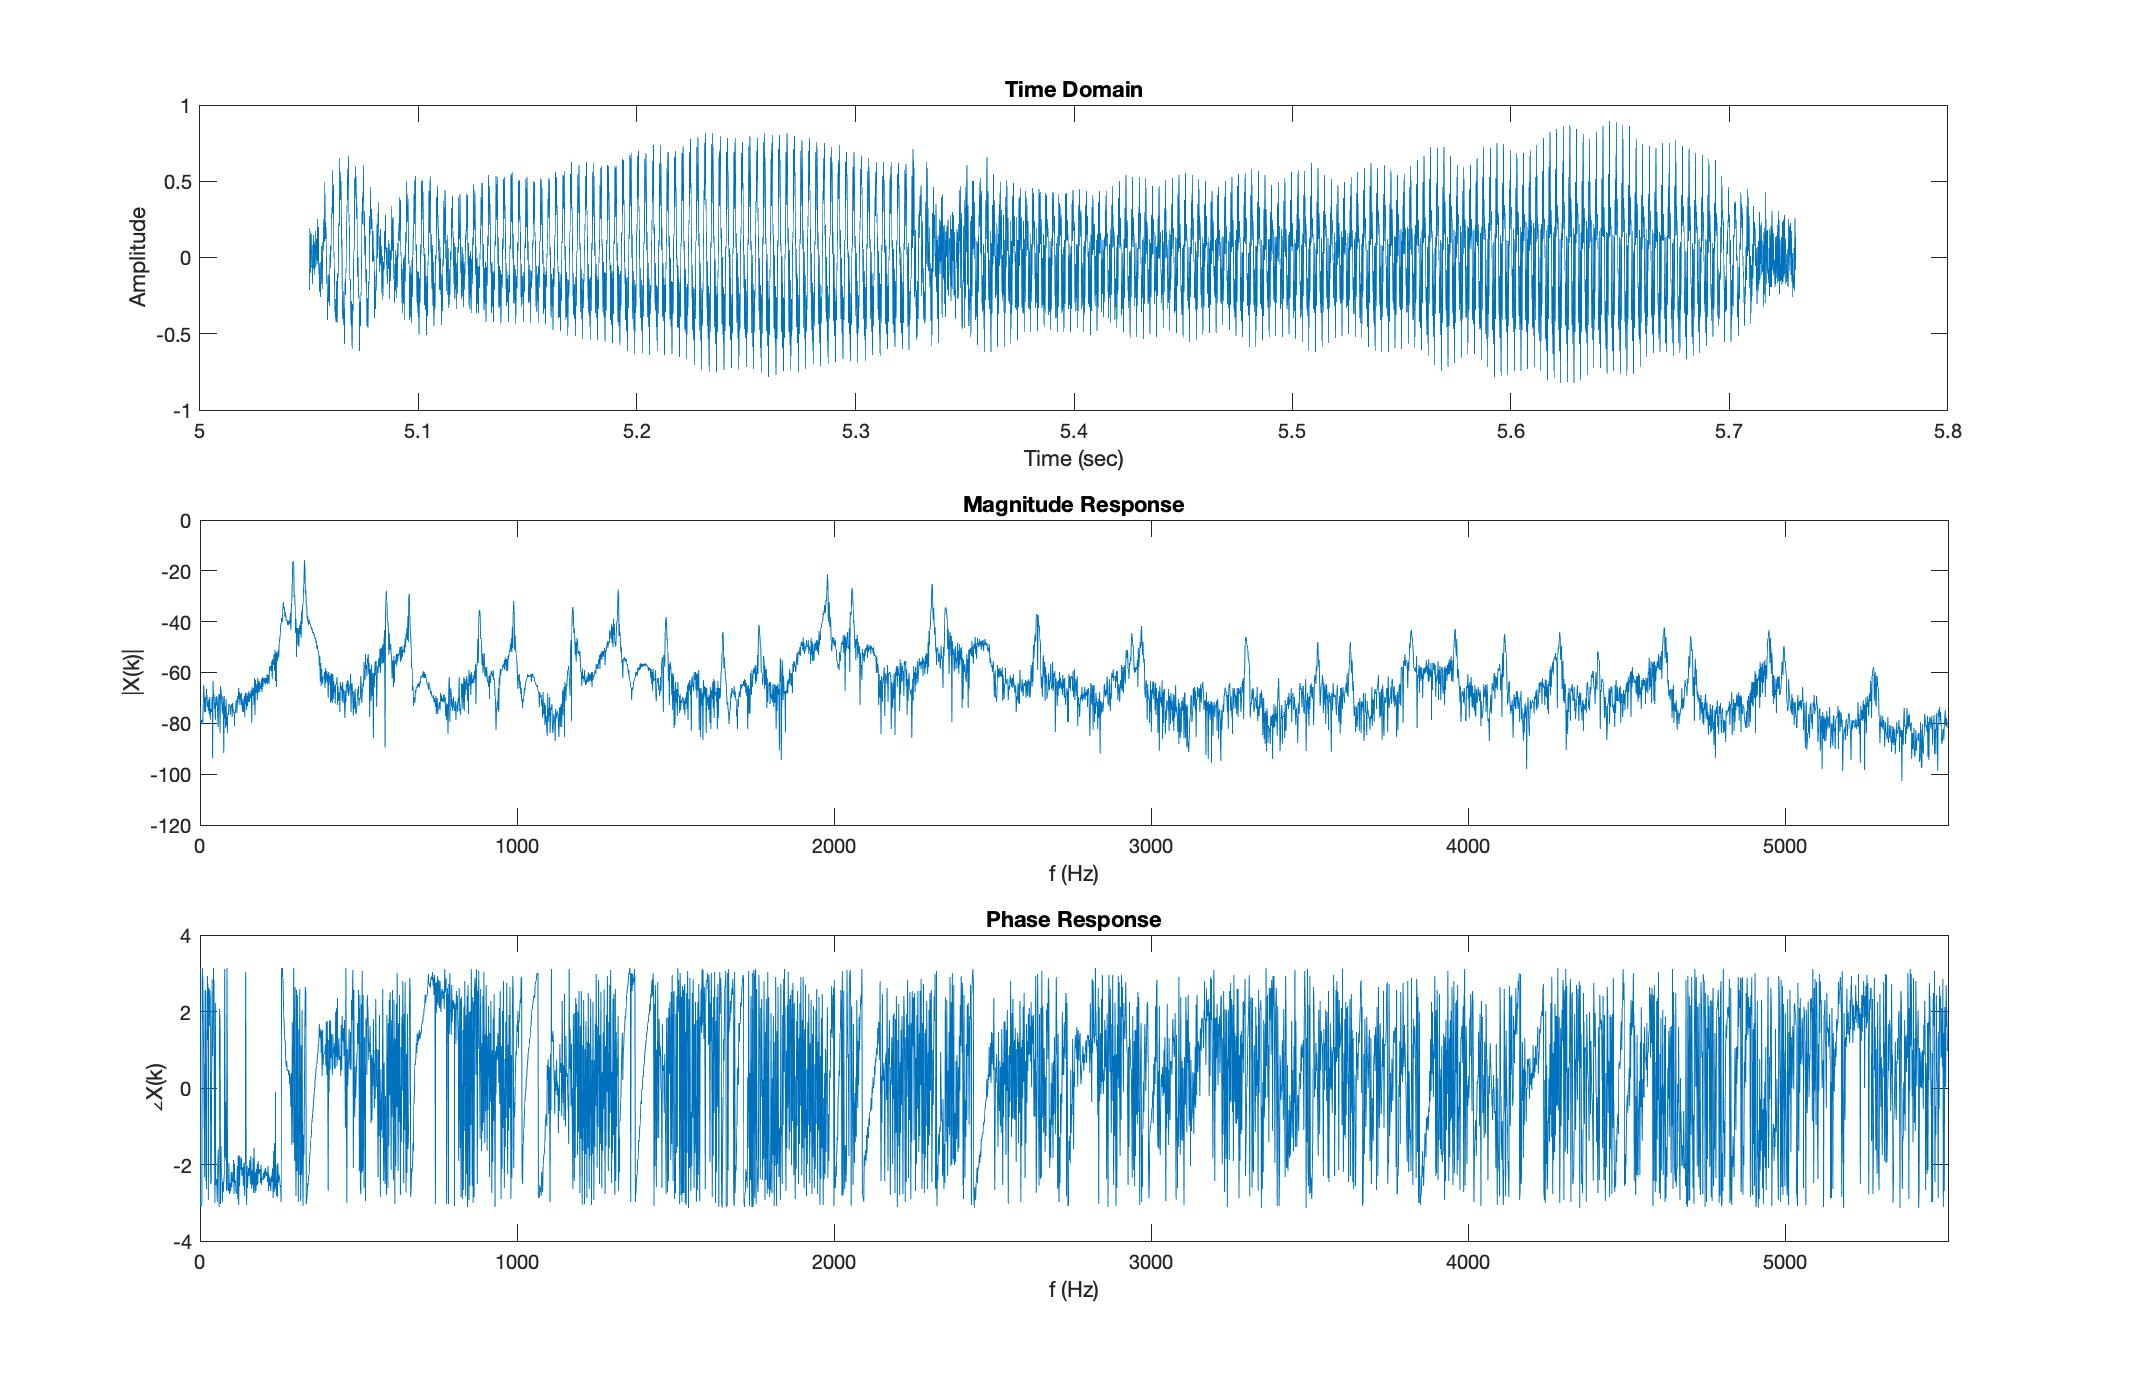
\includegraphics[scale = 0.22]{violinTwoNotes.jpg}
	\end{center}
\end{figure}

If we examine the magnitude response, we can see a set of two repeating peaks starting around 290Hz.  Using the
same intuitions from earlier, it would be logical to surmise that we have two notes playing with fundamentals around
290Hz and slightly higher at, say, 330Hz.  Though it is difficult to tell from Figure \ref{fig:violinTwoNotes}, those peaks
occur at exactly frequency bins 294Hz and 330.8Hz, both very close to the notes D4 and E4 respectively.  Indeed, it is
true that the violin plays those two notes from 5.05 to 5.75 seconds.  However, the magnitude response fails
to indicate whether those notes are successive or chordal.  The time domain, nevertheless, provides some clues.  We 
can see two distinct notes starting at 5.1 seconds and 5.35 seconds suggesting 
that the notes are played successively.  Choosing a large $N$ like 30000 in this example
unfortunately captured two distinct musical moments and merged the frequency content of both notes into one 
magnitude spectrum.  This is an example of where poor time resolution creates confusing magnitude spectra.  A better
solution to this problem would be to use the DFT twice to analyze each note separately.  This would require smaller $N$,
and in turn our frequency resolution would be poorer.  One nice thing about the magnitude response shown in 
Figure \ref{fig:violinTwoNotes} is that the peak frequency bins are almost exactly the frequency of the original note,
making it easy to determine the fundamentals.  Reducing $N$ would potentially move the frequency bins farther away
from those fundamentals.  This is tradeoff we must make when choosing a size for $N$.  

As a general rule, if the audio file has a slow changing spectrum like ambient music, choose a larger $N$.  The issues
related to time resolution will be mitigated if the audio experiences relatively little change in the time domain.  If the 
audio file has fast music, then use a smaller $N$.  Though the frequency resolution will be poorer, a larger $N$ will
simply capture too many musical events to parse.  